\section{System Usage}
\label{sec:usage}

The \code{InitiatorArtifact} loads the configuration contained in
\code{simulation.yaml}, which must me located in the current working directory.
The file is a configuration file using the \code{yaml} syntax and contains
information about the world, people and hovering information that must be
present in the system. An example is:

\begin{lstlisting}
World:
  width: 800
  height: 800

Simulation:
  gui_width: 800
  gui_height: 800
  gui_refresh_rate: 500
  dissemination: 'random'
  dissemination_param: 0.8

Analysis:
  analysis_rate: 1000

People:
  - name: 'pippo'
    behaviour: 'random'
    xpos: 10
    ypos: 20
    device_range: 200
    device_storage: 100
  - name: 'pluto'
    behaviour: 'random'
    xpos: 20
    ypos: 10
    device_range: 200
    device_storage: 100

Hovering:
  - name: 'gentoo_store'
    xanchor: 20
    yanchor: 70
    anchor_radius: 150
    data_size: 10
    data: "If it moves, compile it!"
  - name: 'google_store'
    xanchor: 400
    yanchor: 400
    anchor_radius: 150
    data_size: 20
    data: "Don't be evil!"
  - name: 'apple_store'
    xanchor: 100
    yanchor: 400
    anchor_radius: 100
    data_size: 40
    data: "Think Different!"
\end{lstlisting}

By starting the JASON system, the initiator agent creates the other agents and
starts the system.

Figure~\ref{fig:screens1},~\ref{fig:screens2},~\ref{fig:screens3}
and~\ref{fig:screens4} show screenshots of the running system. The purple
lines that connect people with the hovering information anchors, assert that the
mobile node contains an piece of the hovering information. The size of the hovering
information, related to the mobile node capacity, is shown as a colorful bar inside
the mini-buffer at each people side.

A grey dotted line joining two peoples, indicates that the respective mobile
nodes communicated in the last two seconds.

\begin{figure}[!h]
  \centering
  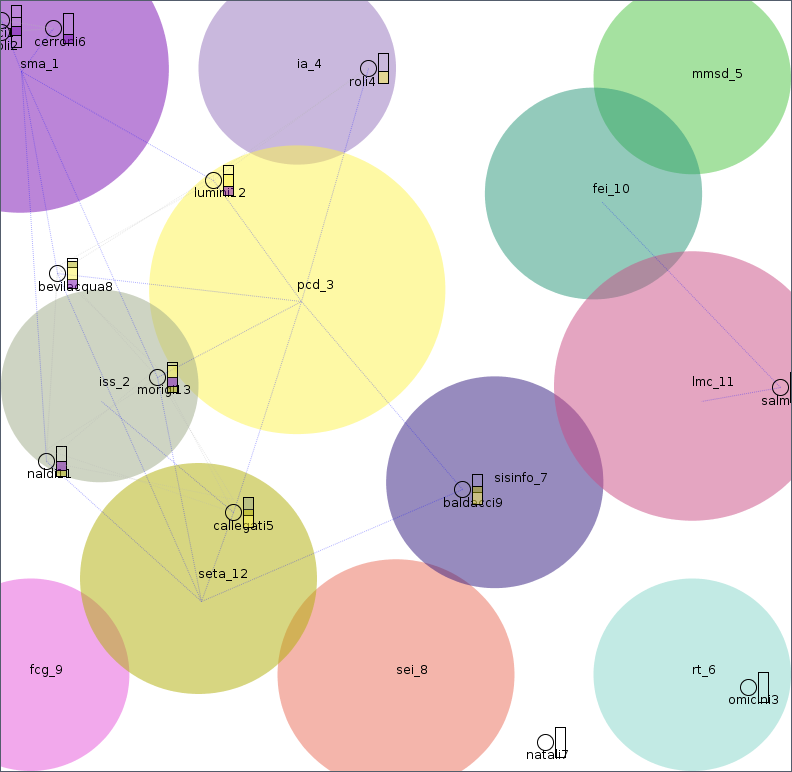
\includegraphics[width=13cm]{./imgs/screen1.png}
  \caption{Screenshot 1}
  \label{fig:screens1}
\end{figure}

\begin{figure}[!h]
  \centering
  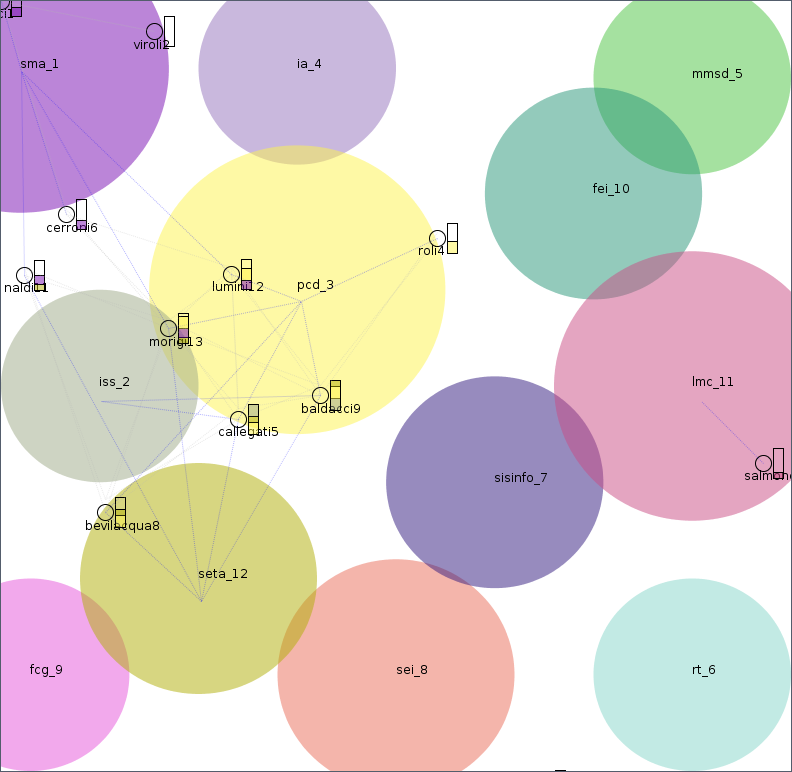
\includegraphics[width=13cm]{./imgs/screen2.png}
  \caption{Screenshot 2}
  \label{fig:screens2}
\end{figure}

\begin{figure}[!h]
  \centering
  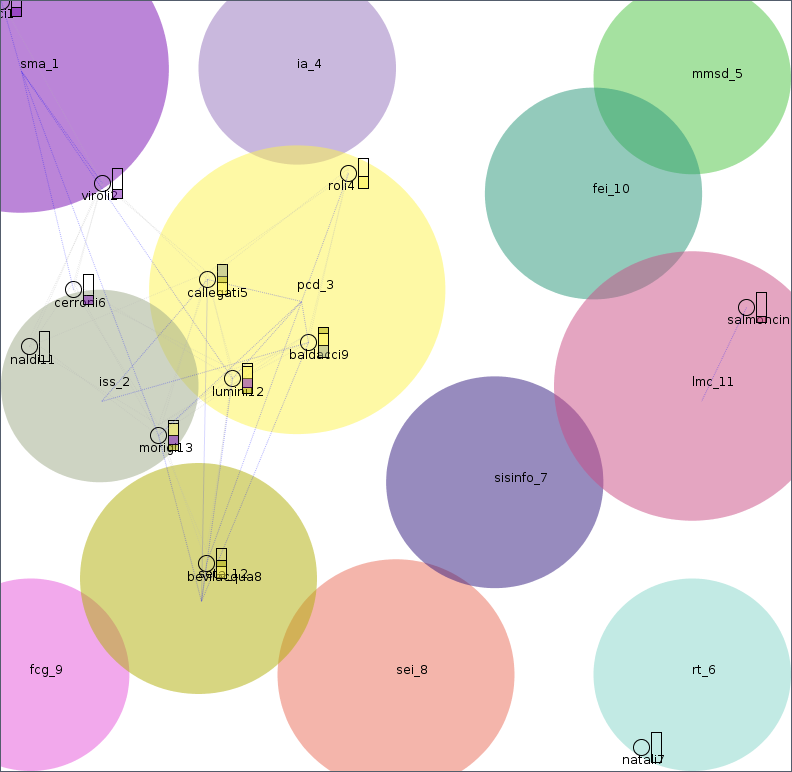
\includegraphics[width=13cm]{./imgs/screen3.png}
  \caption{Screenshot 3}
  \label{fig:screens3}
\end{figure}

\begin{figure}[!h]
  \centering
  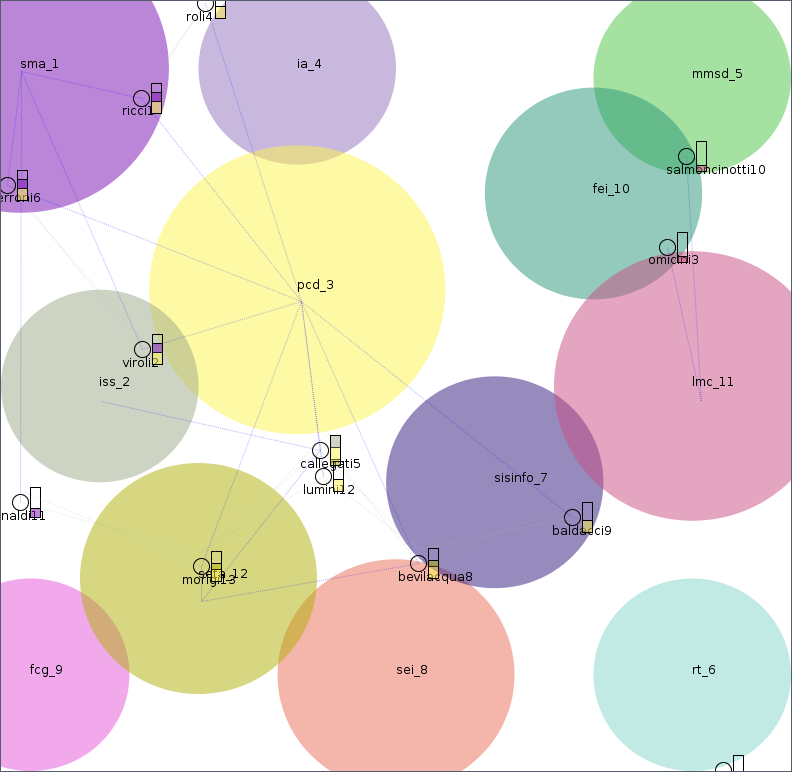
\includegraphics[width=13cm]{./imgs/screen4.png}
  \caption{Screenshot 4}
  \label{fig:screens4}
\end{figure}

\FloatBarrier
